223. \begin{figure}[ht!]
\center{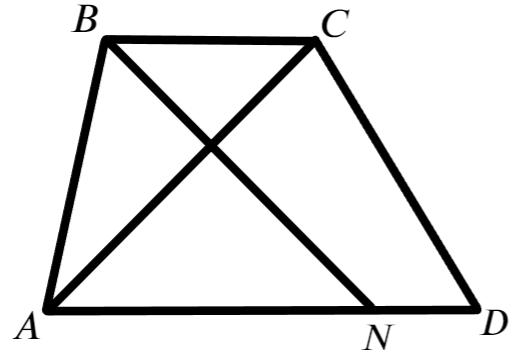
\includegraphics[scale=0.35]{g8-223.png}}
\end{figure}\\
Так как высоты, опущенные из вершин $B$ и $C$ треугольников $ABN$ и $ACD,$ равны (они равны высоте трапеции), их площади относятся как основания, к которым эти высоты проведены, то есть $\cfrac{S(\Delta ACD)}{S(\Delta ABN)}=\cfrac{AD}{AN}=\cfrac{4}{3},$ откуда $S(\Delta ACD)=\cfrac{4}{3}\cdot6=8.$\\
